\section{Results}
\label{sec:results}
All numbers in this section are generated from the stored result files (\texttt{CLAIMS.md} lists each one). Intervals are 95\%
unless stated, from resampling the \nTestSigners{} test signers. Seeds are averaged first. ``Examples per sign'' $k$ means
references for the nearest-neighbour methods and training examples for the learned models; ``all'' uses every training video of
the sign.

\subsection{Main comparison}
\begin{table}[t]
\centering\small
\begin{tabular}{lrrrrrr}
\toprule
Method & 1 & 2 & 5 & 10 & 20 & all \\
\midrule
DTW 1-NN & 17.2 & 22.1 & 31.0 & 38.6 & 45.9 & 63.4 \\
Euclidean 1-NN & 18.9 & 24.7 & 35.0 & 42.7 & 47.5 & 63.2 \\
DBA prototype & 17.2 & 15.2 & 13.4 & 13.1 & 12.7 & 12.4 \\
1D-CNN & 23.2 & 32.0 & 48.2 & 61.1 & 71.6 & 85.5 \\
BiGRU & 20.0 & 28.7 & 43.9 & 56.7 & 67.9 & 84.9 \\
Transformer & 23.7 & 30.3 & 45.9 & 57.0 & 66.2 & 85.9 \\
BiGRU + aug. & 21.9 & 28.5 & 44.5 & 57.9 & 67.7 & 85.1 \\
\bottomrule
\end{tabular}

\caption{Top-1 accuracy (\%) at a vocabulary of 50 signs on the 8 held-out test signers, by examples per sign
(feature set F1, preprocessing chosen per method on validation signers). Intervals are in
\texttt{results/tables/main\_top1.md}.}
\label{tab:main50}
\end{table}
\begin{figure*}[t]
\centering
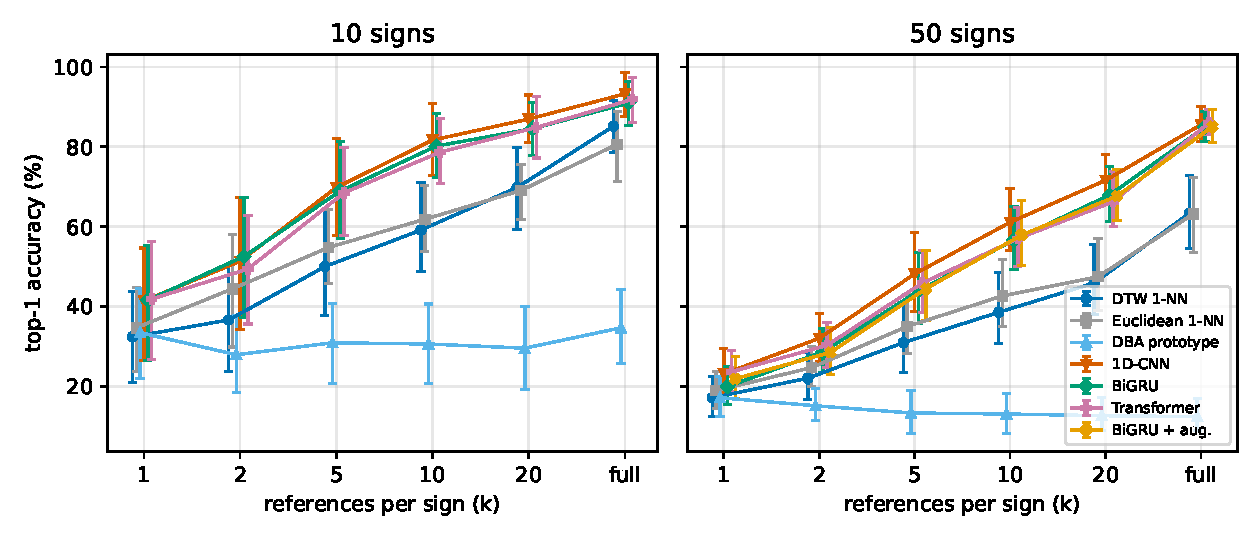
\includegraphics[width=\textwidth]{../figures/accuracy_vs_k.pdf}
\caption{Top-1 accuracy versus examples per sign for vocabularies of 10 and 50 signs. Bars are 95\% intervals from resampling
test signers.}
\label{fig:acc}
\end{figure*}
At a vocabulary of 50 signs and 10 examples per sign, the 1D-CNN reaches \accCnnVFiftyKTen\% top-1
(\accLoCnnVFiftyKTen--\accHiCnnVFiftyKTen), the Transformer \accTransVFiftyKTen\% and the BiGRU \accGruVFiftyKTen\%, against
\accDtwVFiftyKTen\% (\accLoDtwVFiftyKTen--\accHiDtwVFiftyKTen) for DTW 1-NN and \accEuclidVFiftyKTen\% for Euclidean 1-NN
(Table~\ref{tab:main50}, Figure~\ref{fig:acc}). With all training videos the learned models reach \accTransVFiftyKAll\%
(Transformer), \accCnnVFiftyKAll\% (CNN) and \accGruVFiftyKAll\% (BiGRU), and DTW \accDtwVFiftyKAll\%. At 10 signs the ordering
is the same: \accCnnVTenKAll\% (CNN) and \accDtwVTenKAll\% (DTW) with all training videos.

\subsection{Pre-registered hypotheses}
\textbf{H1 is not supported.} We expected DTW to beat each learned model at vocabulary 50 with $k\le5$. Instead every learned
model is above DTW at $k=1$, 2 and 5: \nHOneBelowZero{} of the nine paired differences have 97.5\% intervals wholly on the learned model's side of zero (\texttt{results/tables/hypotheses.csv}). For example, at $k=1$ the CNN is \difCnnVFiftyKOne{} points above DTW
(95\% interval \difLoCnnVFiftyKOne{} to \difHiCnnVFiftyKOne{}), and at $k=5$ it is \difCnnVFiftyKFive{} points above
(\difLoCnnVFiftyKFive{} to \difHiCnnVFiftyKFive{}). \textbf{H2 is supported}: with all training videos each learned model is
above DTW by about \difCnnVFiftyKAll{} (CNN), \difTransVFiftyKAll{} (Transformer) and \difGruVFiftyKAll{} (BiGRU) points, and the intervals remain above zero when adjusted for three comparisons (\hTwoAdjSupported).

\subsection{No crossover in the tested range}
We looked for the number of examples per sign at which learned models overtake DTW and found none: at both vocabularies the best
learned model is at or above DTW from $k=1$ upwards (smallest such $k$: \crossoverTen{} at 10 signs, \crossoverFifty{} at 50).
In \nPairedLearnedExcl{} of the \nPairedLearned{} comparisons of a learned model with DTW (3 models, 6 values of $k$, 2 vocabularies) the 95\% interval excludes
zero, and in \nPairedLearnedAhead{} the learned model's point estimate is higher (exploratory; no multiplicity correction). The gap is smallest at $k=1$, where every method is weak: at 50 signs no method
exceeds \accTransVFiftyKOne\% (Transformer, the best) with one example per sign. Euclidean 1-NN is not worse than DTW at 50 signs:
it is ahead by \difEuclidVFiftyKTwo, \difEuclidVFiftyKFive{} and \difEuclidVFiftyKTen{} points at $k=2$, 5 and 10 (intervals exclude zero) and indistinguishable at $k=1$, 20 and ``all'' (\difEuclidVFiftyKOne, \difEuclidVFiftyKTwenty{} and \difEuclidVFiftyKAll{} points). At 10 signs DTW is ahead
of Euclidean 1-NN only with all training videos (\difEuclidVTenKAll{} points for Euclidean minus DTW, interval
\difLoEuclidVTenKAll{} to \difHiEuclidVTenKAll{}).

\subsection{DTW variants}
DBA prototypes (one barycentre per sign) are poor and get worse with more references per sign at 50 signs
(\accDbaVFiftyKOne\% at $k=1$, \accDbaVFiftyKAll\% with all videos), so we do not recommend averaging signer variants into a single
template. On one fixed draw (50 signs, 10 examples per sign, seed 0), exact DTW scores \accDtwSeedZeroVFiftyKTen\%, FastDTW
(radius 1) \accFastDtwVFiftyKTen\% and the original repository's pipeline \accLegacyVFiftyKTen\%; the intervals overlap
completely (\accLoLegacyVFiftyKTen--\accHiLegacyVFiftyKTen\% for the original pipeline), so these variants are not
distinguishable at this sample size. [PENDING: latency comparison]

\subsection{Preprocessing matters more for the template-matching baselines}
On validation signers (50 signs, 10 examples per sign), DTW with the naive default of zero-filled missing hands and raw features
scored \tuneNaiveDtw\%, against \tuneBestDtw\% for the configuration chosen on validation (frames without a hand dropped,
standardised features, band of 8 frames). The learned models were much less sensitive: best validation accuracy with zero-filled
gaps versus the chosen setting was \tuneZeroCnn\% vs \tuneBestCnn\% for the CNN. Every family chose to drop frames without a
detected hand. We give each family its own validation-selected preprocessing so that no method is held back by an arbitrary
default; the naive default would have made the DTW baseline look \tuneGapDtw{} points worse on validation.

[PENDING: feature ablations, missing-hand and handedness ablations, augmentation arm, one- versus two-handed signs, per-sign errors,
latency]
